\section{Classes and Events}
\label{cap:classesevents}
In the process of finding classes and events we made up several classes and events some of which are not used in the actual program. To come up with the classes and events we talk about different possible scenarios and based on that we developed our class diagram. This section describes all the classes and events in the final iteration of the process and all the redundant classes and events are omitted. On figure \ref{fig:classeseventstable} the relations between classes and events are illustrated.  

\begin{figure}
\begin{center}
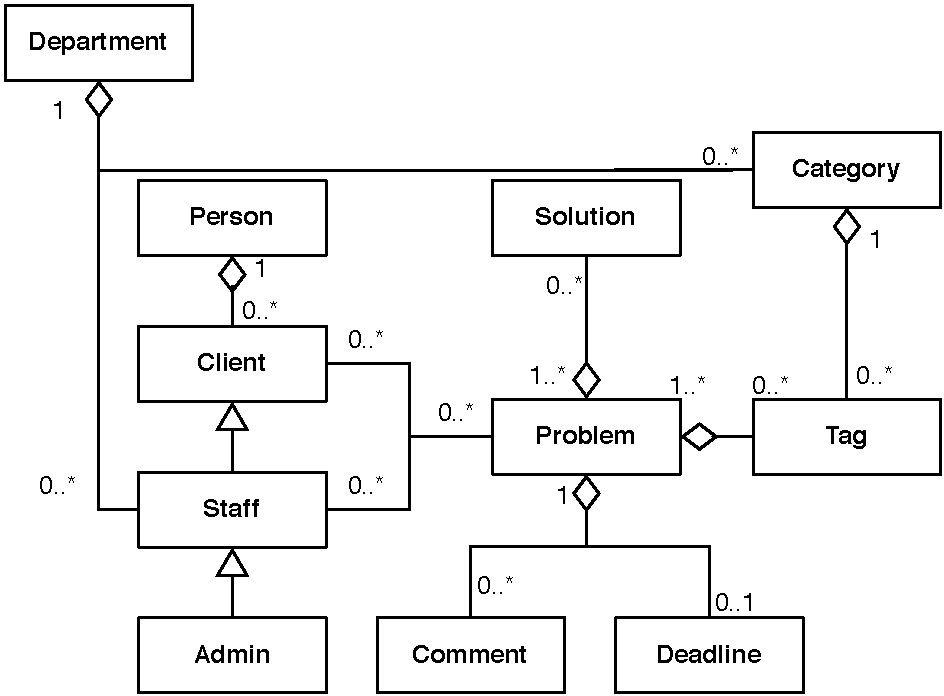
\includegraphics[scale=0.6]{input/problem_domain_analysis/newest_class_diagram.pdf}
\caption{Class diagram}
\label{fig:pdaclassdiagram}
\end{center}
\end{figure}

\subsection{Classes}
The following is a list of the classes from the class diagram \ref{fig:pdaclassdiagram}.

\paragraph{Problem}
Problem is the basic building brick in our system. It is used to hold information about the specific problems which it represents.

\paragraph{Deadline} The deadline can be approved or not approved and is a part of the problem. 

\paragraph{Comment} A comment belongs to a problem. 

\paragraph{Solution}
Contains state and information about a given solution

\paragraph{Person}
This contains attributes about the users in the system, name, address, phone number ect. We will look into the details later in the report.

\paragraph{Client} A \aclient[] can be subscribed to a problem and be associated with the comments that the actor \aclient[] posts.  
 
\paragraph{Staff}
The \astaff[] class inherits from the \aclient[] class.
\astaff[] can be assigned to problems. 

\paragraph{\Admin[]} The \admin[] is not associated with any other classes and is only used to administrate the users. 

\paragraph{Department}
Contains information about staff and categories. 

\paragraph{Category} Categories contain Tags

\paragraph{Tag} Tags is used to determine the problems category and thereby department. 
%\paragraph{List}
%Should contain a list of problems, we choose not to include this class in the project.


%beskriv hvor og hvordan vores problemer bliver opbevaret
\begin{comment}
\subsection{Events}

\paragraph{Problem added}
This event occurs when a user has submitted a problem.

\paragraph{Problem solved}
Occurs when an event receives status of \"solved\".

\paragraph{Problem updated}
Occurs when the content of an event is altered.

\paragraph{Problem assigned}
This event occurs when the problem is assigned to a member of staff.

\paragraph{Problem unassigned}
This event occurs when the problem is unassigned from a member of staff.

\paragraph{Problem deleted}
When a problem is deleted. 

\paragraph{User replied}
An event that occurs when the user replies to something the system has sent him.

\paragraph{Staff replied}
An event that occurs when the staff-member replies to something the system has sent him.

\paragraph{Department created}
An event that occurs when a new department is created.

\paragraph{Department closed}
An event that occurs when a department is closed.

\paragraph{Role assigned}
Occurs when a person has received a new role. We later found that this event was redundant with Staff employed, and decided not to use it.

\paragraph{Role unassigned}
Occurs when a person has lost a role. We later found that this event was redundant with Staff fired, and decided not to use it.

\paragraph{Person created}
This event occurs when a new 

\paragraph{Staff employed}
This event occurs when a person is employed as a staff.

\paragraph{Staff fired}
Event that occurs when a staff-member is fired.

%\paragraph{Solution found:}
%This event triggers when a solution is 
\paragraph{Solution assigned}
This event triggers when a solution is assigned to a problem.

\paragraph{Problem categorized}

This event occurs when a problem is tagged.
\end{comment}

\begin{figure}[]
\begin{tabular}{ l c c c c c} \hline
\\
&\emph{\textbf{Classes}} &  &  & &  \\ 
\emph{\textbf{Events}} & Problem & Solution & Staff & Department & Person \\ \hline
 Problem added 				& $ \checkmark $ &  &  & $ \checkmark $ &  \\ 
 Problem solved 			& $ \checkmark $ & $ \checkmark $ &  & $ \checkmark $ &  \\ 
 Problem updated 			& $ \checkmark $ &  & $ \checkmark $ & $ \checkmark $ &  \\ 
 Problem assigned 		& $ \checkmark $ &  & $ \checkmark $ & $ \checkmark $ &  \\ 
 Problem unassigned 	& $ \checkmark $ &  & $ \checkmark $ & $ \checkmark $ &  \\ 
 Problem deleted 			& $ \checkmark $ &  &  & $ \checkmark $ &  \\ 
 User replied 				& $ \checkmark $ &  & $ \checkmark $ & $ \checkmark $ &  \\ 
 Staff replied 				& $ \checkmark $ &  &  &  &  \\ 
 Department created 	&  &  &  & $ \checkmark $ &  \\ 
 Department closed 		&  &  &  & $ \checkmark $ &  \\ 
 Role assigned 				&  &  &  & $ \checkmark $ & $ \checkmark $  \\ 
 Role unassigned 			&  &  &  &  $ \checkmark $  & $ \checkmark $ \\ 
 Person created 			&  &  &  &  & $ \checkmark $ \\ 
 Solution found 			& $ \checkmark $ & $ \checkmark $ & $ \checkmark $ &  & $ \checkmark $ \\ 
 Solution assigned		& $ \checkmark $ & $ \checkmark $ & $ \checkmark $ &  & $ \checkmark $ \\ 
 Problem categorized	& $ \checkmark $ &  &  & $ \checkmark $ &  \\ \hline
\end{tabular}
\morscaption{Problem-domain analysis event table}
\label{fig:classeseventstable}
\end{figure}

\fixme{sl\aa events sammen, tilf\oe g de nye events, flere classes se klass diagram, fjern urelevante, kald den general, kontroller at checkmarks er sat rigtigt (department)}